\documentclass[onecolumn,aps,prl,superscriptaddress,longbibliography]{revtex4-2}
\setcounter{secnumdepth}{3}
\usepackage[colorlinks,bookmarks=false,citecolor=blue,linkcolor=red,urlcolor=blue]{hyperref}
\usepackage{verbatim}
\usepackage{color}
\usepackage{amsmath,amssymb,bm,braket,float,mathtools}
\usepackage{unicode-math}
\usepackage{graphicx,xfrac,appendix}
\usepackage[english]{babel}
\usepackage{physics}
\usepackage{ctex}
\usepackage{bbm}
\usepackage{subfigure}
\usepackage{epstopdf}

\begin{document}

\title{强度谱学的 $\cos$ 偶性盲区：\\Bragg 谱与谱函数在何种精确意义上分不清 retraced 与 winding 轨迹}
\author{Kun Pu}
\email{kunpuphy@zjnu.edu.cn}
\affiliation{Department of Physics, Zhejiang Normal University, Jinhua 321004, China}
\date{\today}

\begin{abstract}
本笔记确证并精确化如下命题：在一维二能级系统中，Bragg 谱以基态 Bloch 矢量 $\hat{\mathbf{d}}(k_0)$ 为参考轴，确实比以固定 $z$ 轴为参考的对角谱函数（SPSF）多出一个自由维度；但两种探针的\textbf{强度}信号都是\textbf{带符号大圆角度的余弦}——SPSF 为 $\pi\big(1\pm\cos\Phi(k)\big)$，Bragg 为 $\tfrac{N}{2}\big(1\pm\cos(\Phi(k)-\Phi(k_0))\big)$——而 $\cos$ 是偶函数，角度的符号（轨迹走哪一侧、朝哪个方向）从不进入信号。由此得到四个盲区定理：(T1) 对角 SPSF 对绕 $z$ 直径的折叠全盲：winding 轨迹 $\Phi(k)$ 与其原路返回 $|\Phi(k)|$（共享 $d_z$ 与 $r$）逐点同权、同 $\pi$ 穿越读数；(T2) 当参考点为极点（$d_y(k_0)=0$）时 $\cos\Theta=\pm\hat d_z$，Bragg 逐点退化为 SPSF——完全同盲，而 Kitaev 链族的天然 BEC 点 $k_0=0$ 恰为极点；(T3) 全局镜像 $d_y\to-d_y$（$\nu\to-\nu$）保持一切强度不变——绕数\textbf{符号}对任何强度测量永不可见；(T4) 对跖点/满转移判据检验的是 $\hat{\mathbf{d}}$ 的\textbf{像}而非带符号扫掠——双程整圆轨迹（$\nu=0$、像 $=S^1$）使 $W_{\max}(k_0)\equiv1$ 对一切 $k_0$ 假阳性。全部结论由 \texttt{codes/verify\_even\_blindness.py} 数值确证（恒等关系达到机器精度，图~\ref{fig:even}）。取向/符号信息只存在于奇宇称 sector（$\sin\Phi$：非对角谱函数与 Bragg 矩阵元的\textbf{相位}、Zak 相位 $\gamma=\pi\nu$），不来自更多强度数据。
\end{abstract}

\maketitle

\section{命题及其精确化}\label{sec:claim}

\textbf{命题（待确证）。}在一维二能级系统中，Bragg 谱的参考轴是基态 Bloch 矢量 $\hat{\mathbf{d}}(k_0)$ 而非固定的 $z$ 轴，确实比谱函数多出一个更自由的考察维度；但两种方法的最终信号里都是 $\cos\theta$ 的形式，而 $\cos\theta$ 是偶函数、区分不了负角度与正角度——因此当 Bloch 球上的轨迹\textbf{从 $\pi$ 到 $0$ 再原路返回 $\pi$}（非拓扑，$\nu=0$）与\textbf{从 $\pi$ 到 $0$ 再到 $-\pi$}（拓扑，$|\nu|=1$）时，两种谱方法都分不清二者的区别。

\textbf{本笔记的结论分三层。}
\begin{itemize}
\item[(i)] \textbf{无条件成立的部分——偶性结构本身}（定理~\ref{thm:t1}、\ref{thm:t3}、\ref{thm:t4}）：一切强度量都是带符号大圆角度的偶函数；特别是绕数的\textbf{符号}对任何强度测量（任意探针、任意参考、任意组合）永不可见，而"像"型判据对双程整圆型 $\nu=0$ 路径必然假阳性。
\item[(ii)] \textbf{命题逐字成立的确切范围}（定理~\ref{thm:t2}）：当 Bragg 的参考点落在折叠轴上（大圆极点，$d_y(k_0)=0$）时，Bragg 权重逐点退化为 SPSF 权重，与谱函数\textbf{完全同盲}；而 Kitaev 链族的天然 BEC 点 $k_0=0$ 恰为极点（$\mathbf{d}(0)=(0,0,-\mu/2-J)$）。
\item[(iii)] \textbf{诚实的边界}：参考点离开极点后，Bragg 确能分辨这一特定对偶（这正是前记中 $d_y=\cos k$ 弧模型被分辨的原因）；但它读出的仍是轨迹的\textbf{无符号几何}（像），而非带符号绕数（定理~\ref{thm:t4}），且对 $\nu\leftrightarrow-\nu$ 依旧全盲（定理~\ref{thm:t3}）。
\end{itemize}
因此，"\textbf{本质在 $\cos$ 的偶性}"这一判断无条件正确；"Bragg 与谱函数一样分不清"在自然实验配置（极点参考）下逐字成立，在一般参考点下应按 (iii) 精确化为"\textbf{读像不读绕数、读 $|\nu|$ 不读符号}"。记号沿 \texttt{main.tex}；数值实现 \texttt{codes/verify\_even\_blindness.py}，图件 \texttt{fig/even\_blindness.pdf}。

\section{大圆上的带符号角：两种信号的 $\cos$ 形式}\label{sec:setup}

手性一维二能级系统（手性算符 $\Gamma=\sigma_x$，$d_x=0$）的轨迹限制在 $d_y$--$d_z$ 大圆上，用从 $+z$ 轴向 $+y$ 量起的\textbf{带符号角} $\Phi(k)$ 参数化：
\begin{equation}\label{eq:circle}
\mathbf{d}(k) = r(k)\,\big(0,\ \sin\Phi(k),\ \cos\Phi(k)\big),\qquad
\nu = \frac{\Phi(\pi)-\Phi(-\pi)}{2\pi}\ \ (\text{$\Phi$ 连续展开}),
\end{equation}
即绕数是 $\Phi$ 沿闭合回路的\textbf{带符号总扫掠}。本征值 $E_\pm=\pm r$。两种探针的强度信号（\texttt{main.tex} 式 (main\_spsf)、(main\_bragg) 在此几何下的形式）为
\begin{equation}\label{eq:spsf-cos}
A_{\alpha\alpha}(k,\omega) = \pi\big(1+\cos\Phi(k)\big)\,\delta\big(\omega-E_+(k)\big)
+ \pi\big(1-\cos\Phi(k)\big)\,\delta\big(\omega-E_-(k)\big),
\end{equation}
\begin{equation}\label{eq:bragg-cos}
S(q,\omega) = N\Big[\tfrac{1+\cos\Theta}{2}\,\delta_{\rm intra}
+ \tfrac{1-\cos\Theta}{2}\,\delta_{\rm inter}\Big],
\qquad \cos\Theta(k,k_0) = \cos\big(\Phi(k)-\Phi(k_0)\big).
\end{equation}
两个公式都是带符号角（$\Phi(k)$，或 $\Phi(k)-\Phi(k_0)$）的\textbf{余弦}。$\cos$ 偶 $\Longrightarrow$：SPSF 把 $\Phi(k)$ 与 $-\Phi(k)$（大圆上关于 $d_z$ 直径镜像的两点）投影成同一强度；Bragg 把 $\Delta\Phi(k)=\Phi(k)-\Phi(k_0)$ 与 $-\Delta\Phi(k)$（关于\textbf{参考直径}镜像的两点）投影成同一强度。角度的符号——轨迹走哪一侧、朝哪个方向——从不进入任何强度。

\section{四个盲区定理}\label{sec:theorems}

\textbf{定理 1（$z$-折叠盲区 / SPSF）。}\label{thm:t1}
若两个模型逐点共享 $d_z(k)$ 与 $r(k)$，则其对角谱函数~\eqref{eq:spsf-cos} 完全相同。特别地，winding 轨迹 $\Phi(k)$ 与其 $z$-折叠 $|\Phi(k)|$（等价于 $d_y\to|d_y|$，保持 $d_z$ 与 $r$）满足 $\hat d_z=\cos\Phi=\cos|\Phi|$：权重、$\delta$ 线位置、$\pi$ 穿越的位置与个数全部一致——对角 SPSF 把 $\nu=0$ 的原路返回读成 $\nu=1$：\textbf{假阳性}。
\textit{证明：}权重 $\tfrac12(1\pm\hat d_z)$ 只通过 $\hat d_z=d_z/r$ 依赖模型；穿越判据只读 $d_z$ 的符号串。$\blacksquare$

\textbf{定理 2（极点退化 / Bragg）。}\label{thm:t2}
若参考点为极点（$d_y(k_0)=0$，$\hat{\mathbf{d}}(k_0)=\pm\hat z$），则
\begin{equation}\label{eq:pole-deg}
\cos\Theta(k,k_0) = \hat{\mathbf{d}}(k)\cdot\hat{\mathbf{d}}(k_0) = \pm\,\hat d_z(k),
\end{equation}
Bragg 权重逐点化为 SPSF 权重（两个极点之间差一个带内/带间交换），线位置亦同——\textbf{Bragg 完全继承 SPSF 的盲区}，包括定理~\ref{thm:t1} 的一切折叠对。反之，若 $\sin\Phi(k_0)\neq0$，$z$-折叠对的权重差 $\propto\sin\Phi(k)\,\sin\Phi(k_0)$ 在折叠半支上非零：可分辨。故\textbf{retraced/winding 对偶在 Bragg 下不可分辨 $\iff d_y(k_0)=0$}。Kitaev 链 $\mathbf{d}(0)=(0,0,-\mu/2-J)$：天然 BEC 点 $k_0=0$ 恰为极点。$\blacksquare$

\textbf{定理 3（全局镜像 / 符号盲区）。}\label{thm:t3}
替换 $d_y(k)\to-d_y(k)$（$\Phi\to-\Phi$，含参考点；$d_z$、$r$、$E_\pm$ 与基态赝自旋结构不变）使 $\nu\to-\nu$，而 SPSF 的 $\cos\Phi(k)$、Bragg 的 $\cos(\Phi(k)-\Phi(k_0))$ 以及任何由 Bloch 矢量点积或投影模方构成的强度全部不变。故\textbf{绕数的符号对一切强度数据不可见}。$\blacksquare$

\textbf{定理 4（像 $\neq$ 绕数）。}\label{thm:t4}
满转移判据 $W_{\max}(k_0)=1\iff-\hat{\mathbf{d}}(k_0)\in\mathrm{image}\,\hat{\mathbf{d}}$ 只依赖\textbf{像集}；$\pi$ 穿越数只依赖 $\hat d_z$ 的符号串——两者都不含带符号扫掠。构造\textbf{双程整圆} DC：$\Phi=2k+\pi$（$k\in[-\pi,0]$）、$\pi-2k$（$k\in[0,\pi]$）：$\nu=0$ 而像 $=S^1$，故 $W_{\max}\equiv1$ 对一切 $k_0$ 成立、每带 4 次 $\pi$ 穿越（读作 $\nu=2$）；且 DC 正是真实 $\nu=2$ 模型（$\Phi=2k+\pi$）的 $z$-折叠——二者 SPSF 全同、从一切极点参考 Bragg 全同。$\blacksquare$

\section{显式对偶与数值确证}\label{sec:numerics}

\textbf{对偶（$r\equiv1$，$E_\pm=\pm1$，能量逐点相同）。}
\begin{equation}\label{eq:pair}
\begin{aligned}
&\mathrm{T}:\ \Phi_{\rm T}(k)=-k,\quad \mathbf{d}_{\rm T}=\big(0,\ -\sin k,\ \cos k\big)\ \ [\pi\to0\to-\pi,\ \nu=-1];\\
&\mathrm{R}:\ \Phi_{\rm R}(k)=|k|,\quad \mathbf{d}_{\rm R}=\big(0,\ |\sin k|,\ \cos k\big)\ \ [\pi\to0\to\pi,\ \nu=0].
\end{aligned}
\end{equation}
R 即 T 的 $k>0$ 半支绕 $z$ 直径的镜像（$k<0$ 半支二者重合）——正是命题中"原路返回"与"继续缠绕"的极简实现（图~\ref{fig:even}(a)）。注：R 在 $k=0$ 处有一个折点（动量空间合法、实空间非局域的哈密顿量）；把折点在 $\varepsilon$ 窗口内光滑化，一切信号连续地偏离零差 $O(\varepsilon)$，盲区结论稳定。光滑的同 $d_z$ 折叠（$\mathbf{d}=(0,\sin^2k,\cos k)$）的行为见下表末行。

\textbf{数值确证}（\texttt{verify\_even\_blindness.py}；"恒等"判据阈值 $10^{-12}$）：
\begin{center}
\renewcommand\arraystretch{1.35}
\begin{tabular}{c|l}
\hline
检验 & 结果 \\
\hline
真值 $\nu$ & $\mathrm{T}=-1$，$\mathrm{R}=0$，$\mathrm{T}^*=+1$，$\mathrm{W}_2=+2$，DC $=0$ \\
T1：SPSF，$\mathrm{T}$ vs $\mathrm{R}$ & $\max|\Delta|=0$（逐点恒等）；每带穿越数 $2=2$（读数 $\nu=1$） \\
T2：Bragg @ $k_0=0$（极点） & $\max|\Delta|=0$（严格）；@ $k_0=\pm\pi$：$\le2.2\times10^{-16}$ \\
T2$'$：Bragg @ $k_0=-\pi/2$ & $k=\pi/2$ 处 T：$\Theta=\pi$ 满转移 $=1$；R：$\Theta=0$ 强度 $=0$（分辨） \\
T3：镜像 $\mathrm{T}$ vs $\mathrm{T}^*$ & SPSF 与一切 $k_0$ 的 Bragg：$\max|\Delta|=0$ \\
T4：DC（$\nu=0$，像 $=S^1$） & $W_{\max}(k_0)\equiv1\ \forall k_0$；4 穿越（读作 $\nu=2$）；与 $\mathrm{W}_2$（真 $\nu=2$）\\
 & SPSF 全同、五个极点参考 Bragg 全同（$\le3.3\times10^{-16}$）、一般 $k_0$ 分辨 \\
T2$''$：$\mathrm{R}$ 的 $W_{\max}(k_0)$ & $=1$ 仅在极点 $k_0=0,\pm\pi$；$k_0=-\pi/2$ 处 $=0.5$：假阳性点与盲点重合 \\
联合探针 & 由 $\cos\Phi(k)$ 与 $\cos(\Phi-\Phi_0)$（$\sin\Phi_0\neq0$）重构 $\sin\Phi(k)$ \\
 & 至一个全局符号（误差 $2.2\times10^{-16}$；镜像系统给出同一数据） \\
光滑折叠 $(0,\sin^2k,\cos k)$ & 权重差 $0.057$（$r$ 差 $\Rightarrow$ 线位置差），但穿越数 $2=2$、\\
 & $k_0=0$ 对跖检验 $1=1$ 同触发：判据级假阳性保持 \\
\hline
\end{tabular}
\end{center}

\begin{figure}[H]
\centering
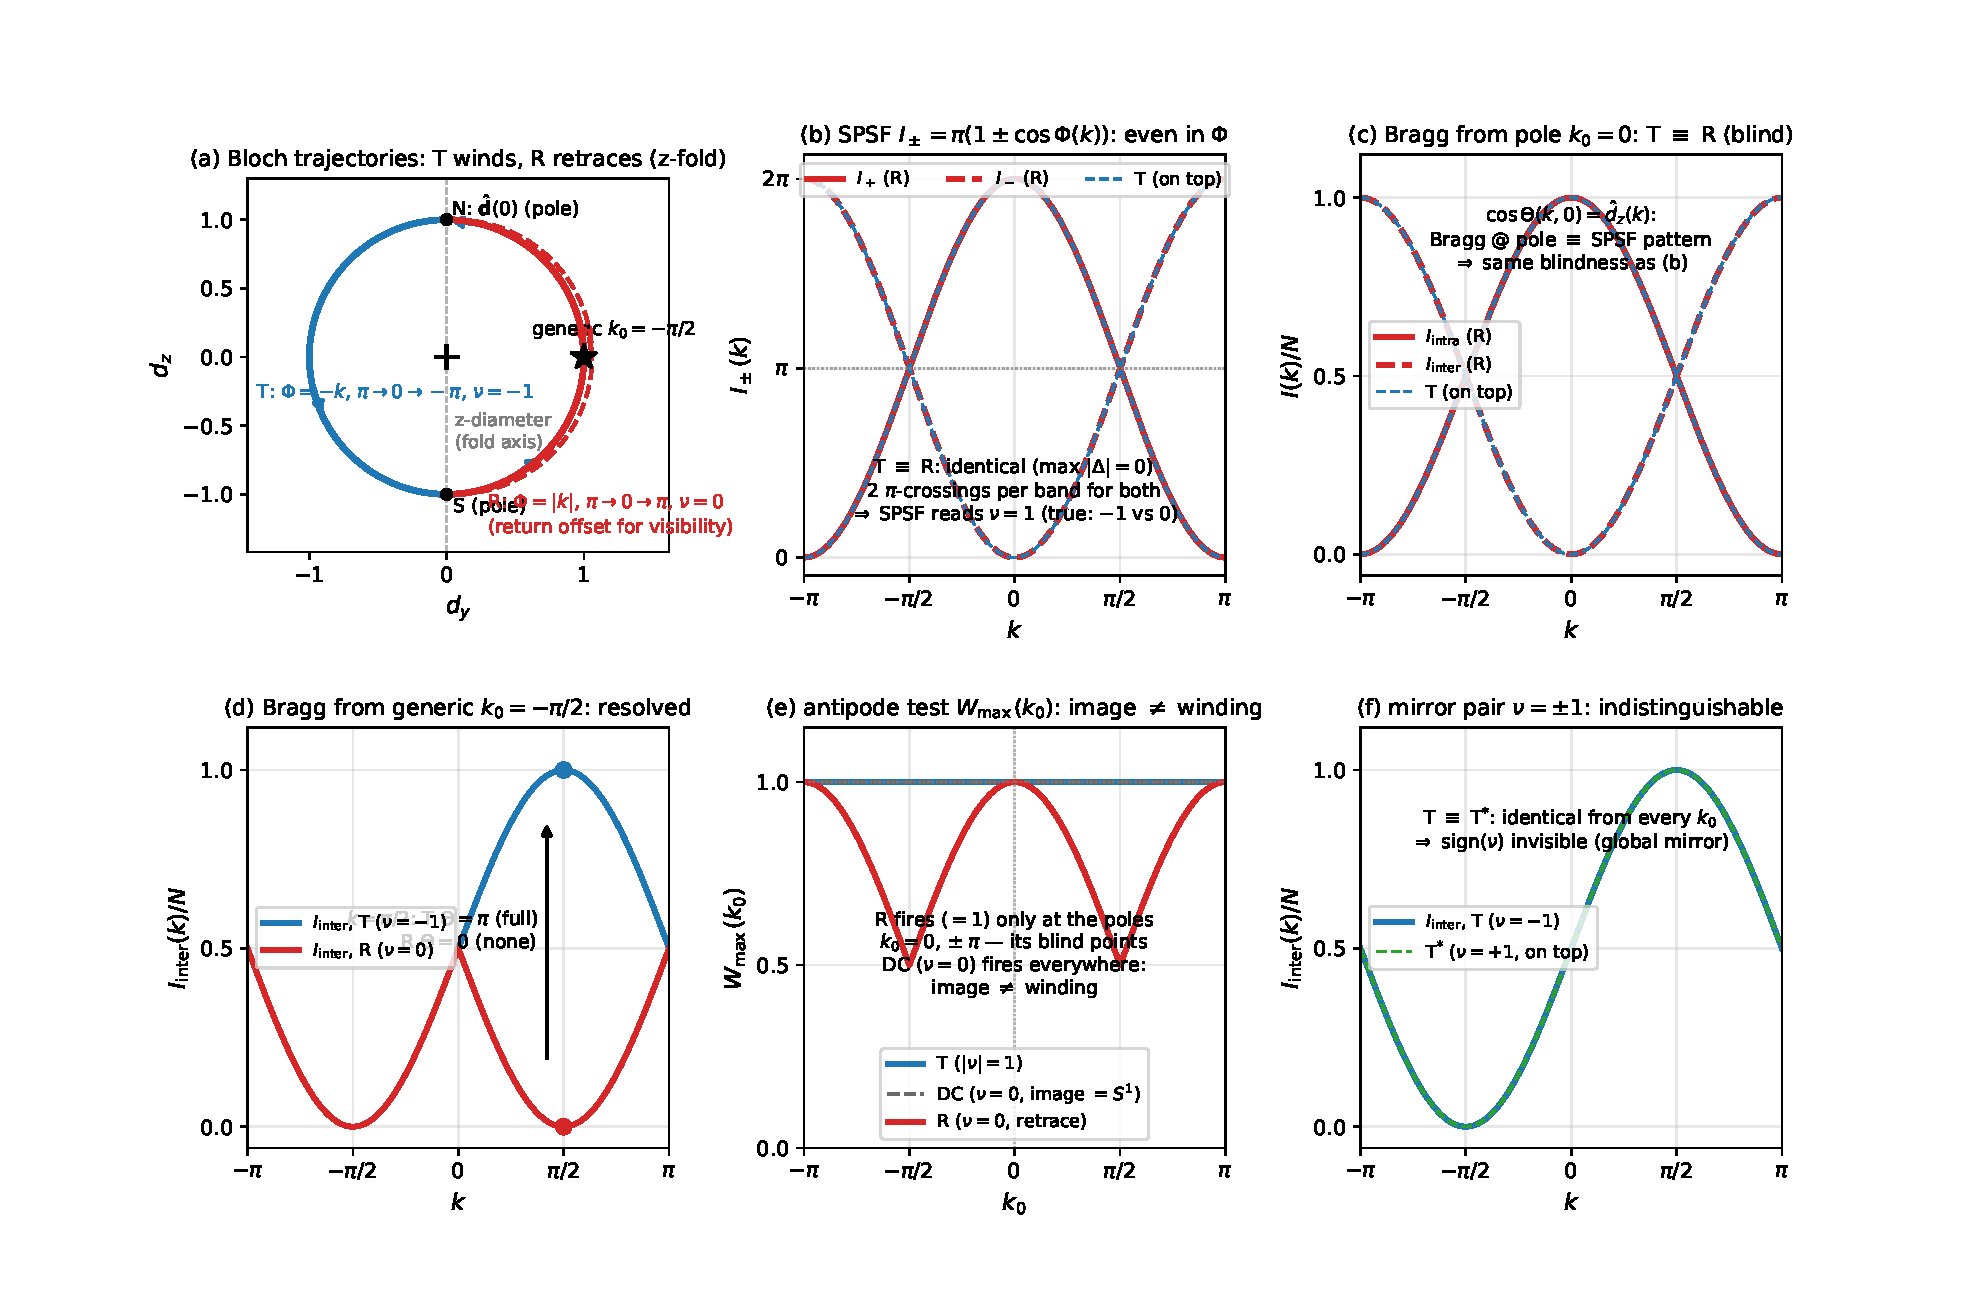
\includegraphics[width=0.98\textwidth]{../fig/even_blindness.pdf}
\caption{六面板总结。(a) 大圆上的对偶：T（winding，$\nu=-1$）与 R（retrace，$\nu=0$；返程曲线为可见性作了平移）；(b) 对角 SPSF 强度 $\pi(1\pm\cos\Phi(k))$——T 与 R 逐点全同，每带 2 次 $\pi$ 穿越，读数 $\nu=1$：假阳性；(c) 极点参考 $k_0=0$ 的 Bragg——$\cos\Theta=\hat d_z$，与 (b) 完全相同：同盲；(d) 一般参考 $k_0=-\pi/2$——$k=\pi/2$ 处 T 满转移（$\Theta=\pi$）、R 零强度（$\Theta=0$）：分辨；(e) 对跖检验 $W_{\max}(k_0)$——R 只在极点（恰为其盲点）触发，DC（$\nu=0$、像 $=S^1$）处处触发：像 $\neq$ 绕数；(f) 镜像对 $\nu=\pm1$ 从任何参考全同：绕数符号不可见。}
\label{fig:even}
\end{figure}

\section{盲区等级、信息所在与三个案例的统一}\label{sec:info}

\textbf{盲区等级。}把"某配置下的数据能确定什么、把什么混为一谈"列表（由定理~\ref{thm:t1}--\ref{thm:t4} 立得）：
\begin{center}
\renewcommand\arraystretch{1.35}
\begin{tabular}{c|c|l}
\hline
探针配置 & 数据确定 & 不可分辨的替换（盲区等价类） \\
\hline
SPSF 对角（固定 $\hat z$） & $\cos\Phi(k)\ \forall k$ & 逐点 $\Phi(k)\leftrightarrow-\Phi(k)$（绕 $z$ 直径的任意折叠） \\
Bragg，极点参考 $d_y(k_0)=0$ & 同 SPSF & 同上（退化为 SPSF，定理~\ref{thm:t2}） \\
Bragg，一般参考 $k_0$ & $\cos(\Phi(k)-\Phi(k_0))\ \forall k$ & 绕 $k_0$ 直径的分段折叠（切换点仅在轨迹过 $k_0$ 直径处） \\
SPSF $+$ 一般参考 Bragg & $\sin\Phi(k)$ 至全局符号 & 仅全局镜像 $\Phi\leftrightarrow-\Phi$：$\nu\leftrightarrow-\nu$ \\
任意强度组合 & —— & $\mathrm{sign}\,\nu$ 永不可见（定理~\ref{thm:t3}） \\
\hline
\end{tabular}
\end{center}
构造性地：$\cos\Theta=\cos\Phi\cos\Phi_0+\sin\Phi\sin\Phi_0$，已知 $\cos\Phi(k)$（SPSF）并取 $\sin\Phi_0\neq0$ 的参考点，即可解出 $\sin\Phi(k)$——但只能到一个\textbf{全局}符号（镜像系统给出同一数据，表中末行）。$|\nu|$ 原则上可定，$\mathrm{sign}\,\nu$ 永不可。

\textbf{三个案例的统一。}前记中的三个结果全部是本笔记定理的实例：
\begin{itemize}
\item \textbf{$\sin^2k$ 模型}（\texttt{main.tex} §1.5 的前身）：$z$-型折叠、$d_z$ 不变，且 $k_0=0$ 为极点（$d_y(0)=0$）$\Rightarrow$ 定理~\ref{thm:t1} $+$ 定理~\ref{thm:t2}：SPSF 与 Bragg \textbf{同时}假阳性（"antipode fires at $\nu=0$"）。
\item \textbf{$\cos k$ 线段模型}（\texttt{main.tex} §1.5）：$k_0=0$ 处 $d_y(0)=\Delta\neq0$，\textbf{非}极点 $\Rightarrow$ 处于定理~\ref{thm:t2} 的边界之外，Bragg 分辨（$W_{\max}<1$）。但如定理~\ref{thm:t4} 所示，这是\textbf{像退化}检验（线段的像不含对跖点），并非读出绕数：对 DC 型 $\nu=0$（像 $=S^1$）的取向抵消同样失效，且由定理~\ref{thm:t3}，它也分不清 $\nu=\pm1$。
\item \textbf{Estake--Roy 二维 QWZ false positive}：天然 BEC 点 $(\pi,\pi)$ 处 $\hat{\mathbf{d}}=\pm\hat z$（极点）$\Rightarrow$ 从该点 Bragg 退化为 SPSF、失效；一般 $k_0$（$W_{\max}\approx0.72<1$）分辨——同为像检验。其论文提出的一阶相干补救（他们的 Eq.~(25)）正是读取下述奇宇称 sector。
\end{itemize}

\textbf{信息所在（奇宇称 sector）。}强度测量丢失的信息恰是 $\sin\Phi$——角度的符号、轨迹的侧别与\textbf{取向}。它只存在于\textbf{相位敏感}的量：
\begin{itemize}
\item \textbf{非对角谱函数}：$A_{\alpha\beta}\propto\hat d_x-i\hat d_y=-i\sin\Phi(k)$——模 $|\sin\Phi|$ 仍是偶函数（模长照样盲），但\textbf{幅角} $\arg A_{\alpha\beta}=\mp\pi/2$（$\sin\Phi$ 的符号）携带折叠/取向信息：一阶相干测量（Estake--Roy 的补救）；
\item \textbf{Bragg 矩阵元的相位}：小 $q$ 极限 $M_{--}(k,k_0)\approx e^{-iq\,\mathcal{A}(k)}$ 给出 Berry 联络；一维手性系统的 Zak 相位 $\gamma=\pi\nu\ (\mathrm{mod}\ 2\pi)$——对式~\eqref{eq:pair} 的对偶给出 $\pi$ vs $0$：相位量直接读到绕数（mod 2）；
\item \textbf{干涉型 Bragg / 时间分辨动力学}：把相位信息转入强度的其他协议。
\end{itemize}

\section{结论}\label{sec:conclusion}

绕数是\textbf{带符号}的拓扑量（取向/手征）；强度是 $\cos$ 型的\textbf{偶}量。偶性盲区是结构性的：它不因参考点的选择、探针的组合或数据量的增加而消失——在极点参考处被逐字满足（定理~\ref{thm:t2}，即 Kitaev 链族的天然配置 $k_0=0$），在一般参考处收窄为全局镜像与像检验（盲区等级表），而 $\mathrm{sign}\,\nu$ 与 DC 型取向抵消对\textbf{一切}强度数据永不可见（定理~\ref{thm:t3}、\ref{thm:t4}）。命题的"本质"——$\cos$ 偶性 $\Rightarrow$ 正负角不分 $\Rightarrow$ retraced 与 winding 不分——由此确证：在自然配置下两种谱方法确实一样分不清；补救不来自更多强度数据，而来自相位/相干测量。

\end{document}
